% 2026 한국상담학회 연차학술대회 공식 포스터 템플릿 (LaTeX 이식)
% 배경: PPTX 템플릿에서 '채움 텍스트'만 제거해 렌더한 assets/template_bg.png (디자인 100% 동일)
% 본문: 원본 PPTX 좌표(EMU→mm)에 textpos로 절대 배치
\documentclass{article}
\usepackage[paperwidth=841mm,paperheight=1189mm,margin=0mm]{geometry}
\usepackage{fontspec}
\setmainfont{NotoSansKR}[Path=../fonts/,
  UprightFont=NotoSansKR-Regular.otf,BoldFont=NotoSansKR-Bold.otf]
\usepackage{graphicx}
\usepackage{tikz}
\usetikzlibrary{shapes.geometric,arrows.meta,positioning}
\usepackage[absolute,overlay]{textpos}
\usepackage{eso-pic}
\usepackage[table]{xcolor}
\usepackage{ragged2e}
\usepackage{booktabs}
\usepackage{tabularx}
\usepackage{enumitem}
\setlist[itemize]{leftmargin=1.5em,itemsep=4pt,topsep=2pt,parsep=0pt}

\setlength{\TPHorizModule}{1mm}
\setlength{\TPVertModule}{1mm}
\setlength{\parindent}{0pt}
\setlength{\parskip}{4pt}
\tolerance=2500
\emergencystretch=3em
\pagestyle{empty}

\definecolor{kcanavy}{RGB}{20,40,90}
\definecolor{txt}{HTML}{2C2C2C}   % 템플릿 본문 색

\newcommand{\titlefs}{\fontsize{80}{90}\selectfont}
\newcommand{\authorfs}{\fontsize{46}{54}\selectfont\bfseries}
\newcommand{\bodyfs}{\fontsize{30}{40}\selectfont}
\newcommand{\subhd}[1]{\par\vspace{2mm}{\fontsize{31}{39}\selectfont\bfseries #1}\par\vspace{2.5mm}}
\newcommand{\figcap}[1]{\par\vspace{1.5mm}{\fontsize{19}{24}\selectfont\color{txt!75}\textit{#1}}\par\vspace{2.5mm}}

% pipeline styles (4-layer refinement flow, full column width)
\tikzset{
  pipe/.style={rectangle, rounded corners, minimum height=18mm, text width=315mm,
    align=center, draw=kcanavy, line width=0.9pt, fill=kcanavy!7,
    font=\fontsize{21}{25}\selectfont, inner sep=3.5mm},
  pipehi/.style={pipe, fill=orange!20},
  parr/.style={-{Stealth[length=5mm]}, line width=1.2pt, draw=kcanavy},
}

\begin{document}

% ---- full-bleed template background (design identical to PPTX) ----
\AddToShipoutPictureBG*{%
  \put(0,0){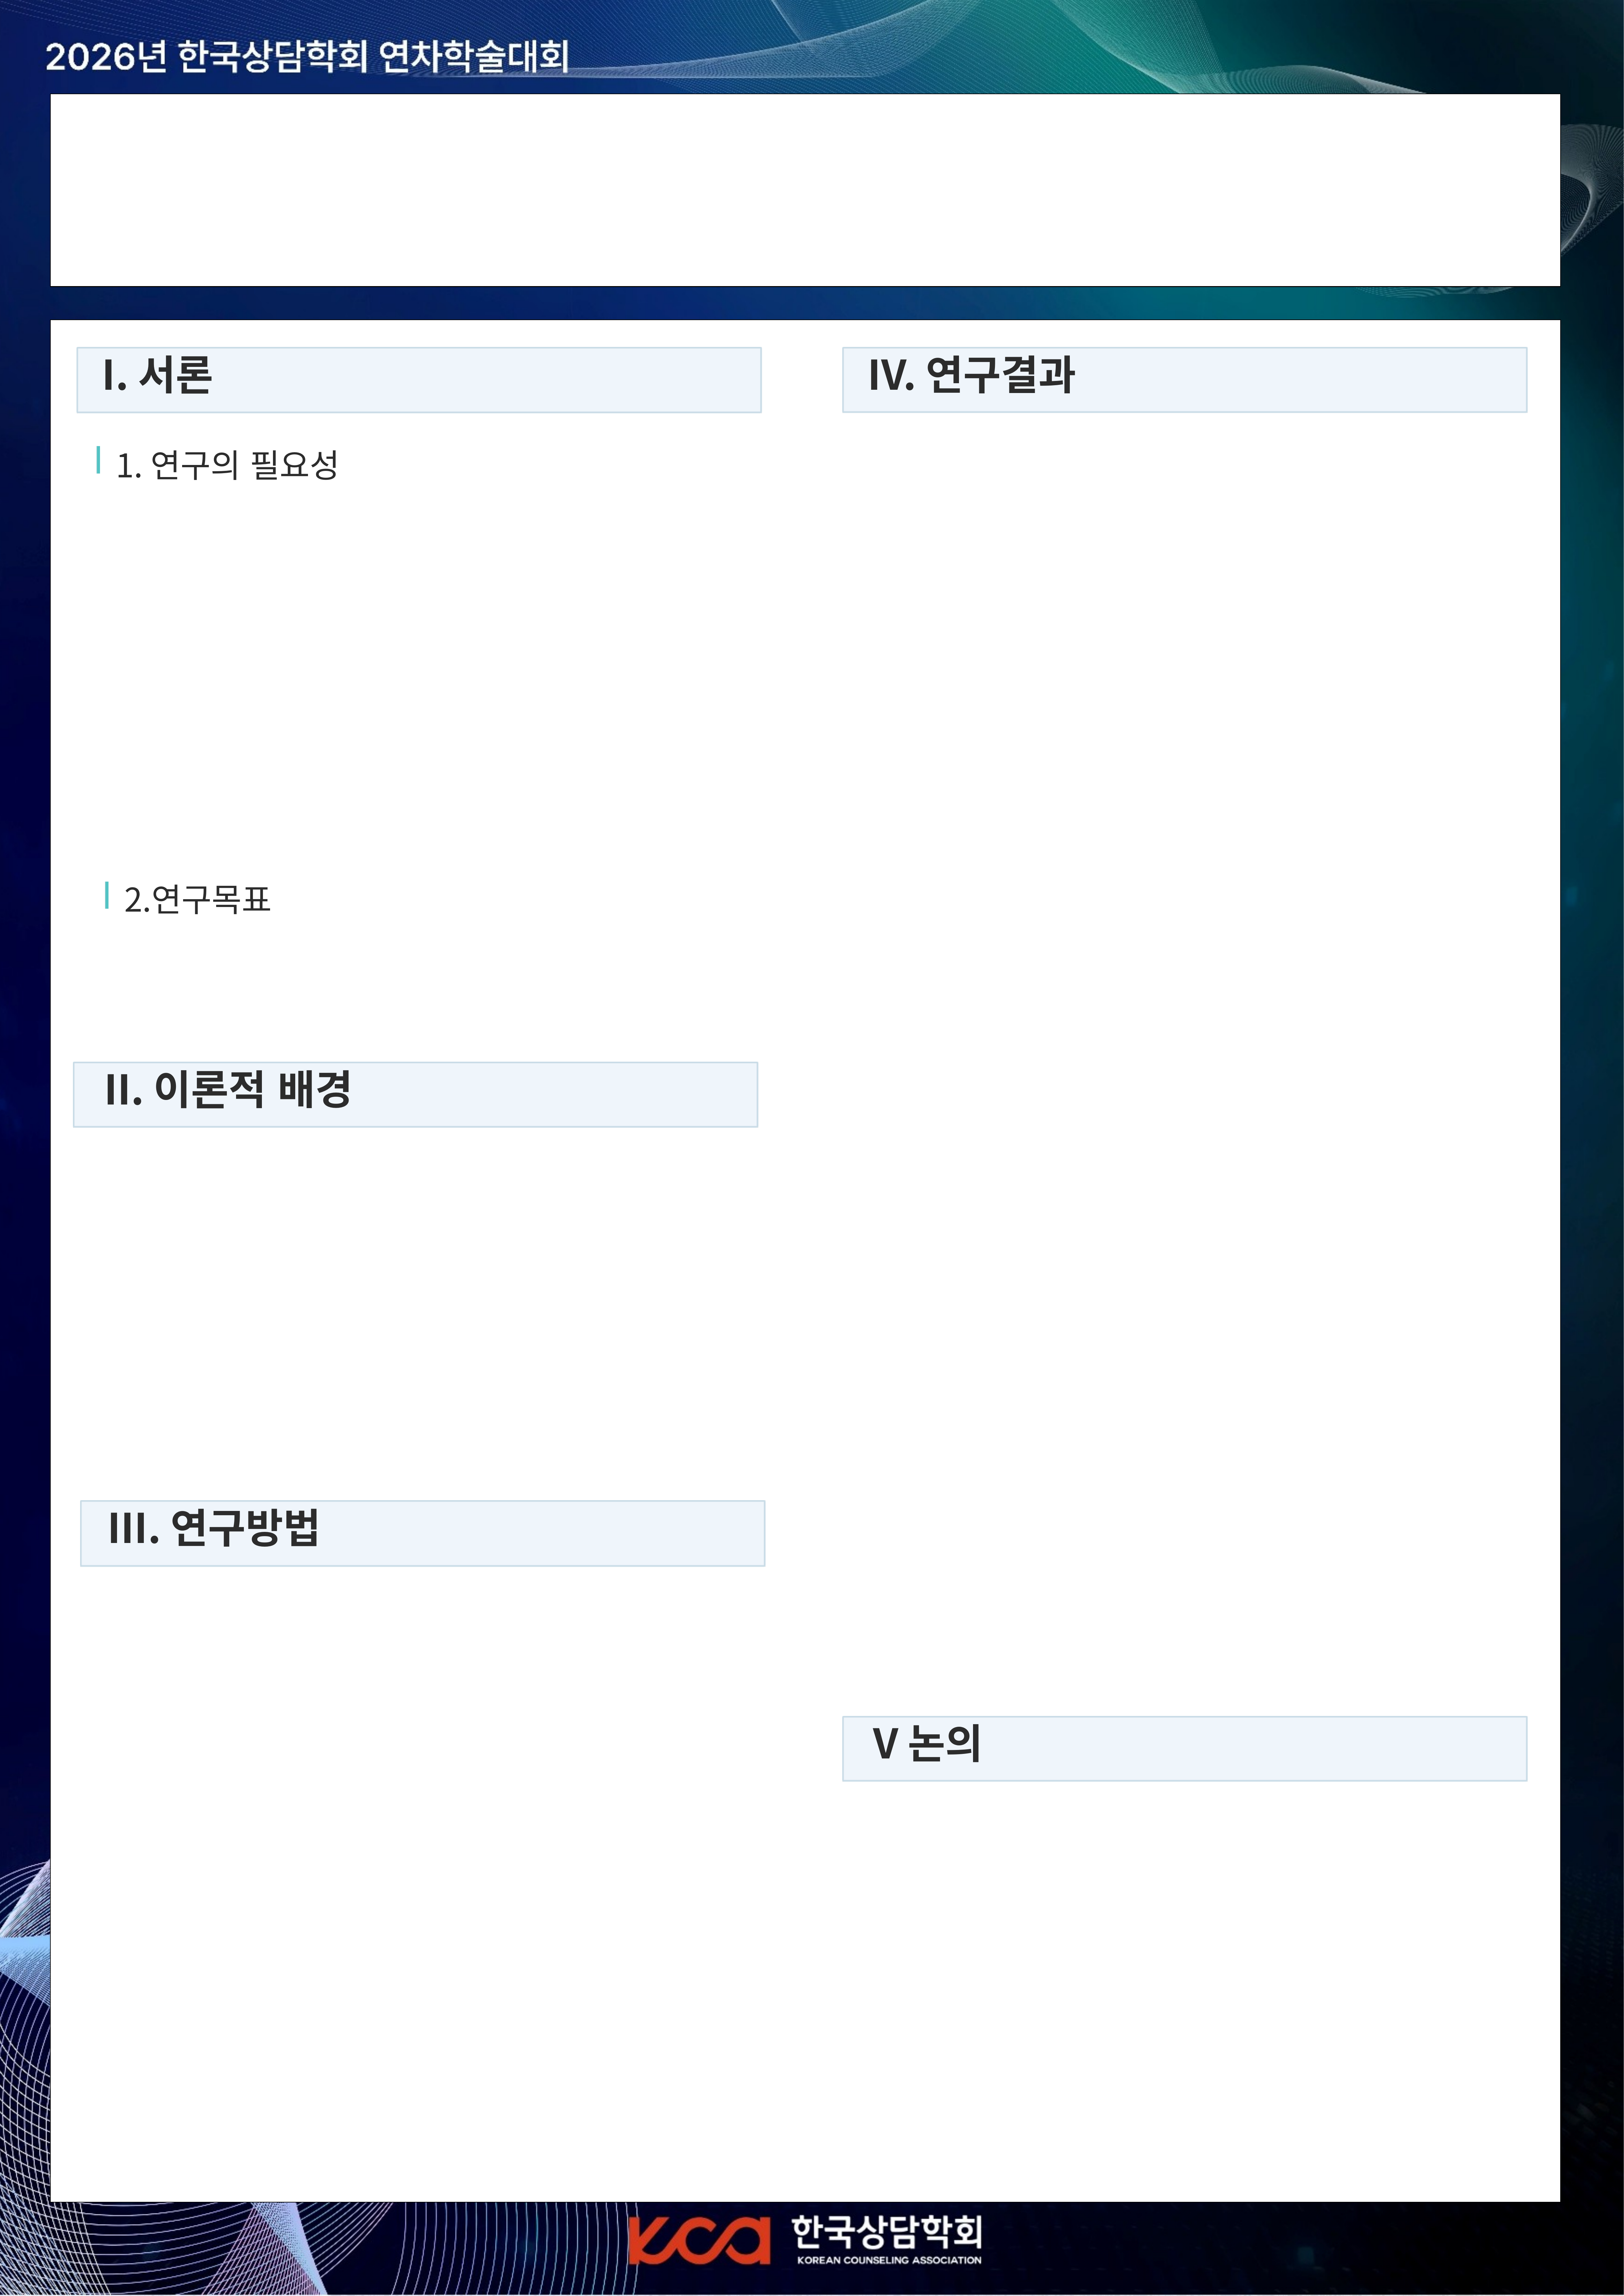
\includegraphics[width=\paperwidth,height=\paperheight]{assets/template_bg.png}}%
}
\color{txt}% 템플릿 본문 색(2C2C2C)

% ===================== TITLE / AUTHOR =====================
\begin{textblock}{701}(70,58)
  \centering\titlefs\textbf{한국어 공개 SNS에 기록된 상담 경험의 기술적 특징}\\[2mm]
  {\fontsize{40}{46}\selectfont LLM 보조 정제 절차로 분석한 사례 보고}
\end{textblock}
\begin{textblock}{701}(70,123)
  \centering\authorfs 이윤정 (서울대학교)
\end{textblock}

% ===================== LEFT COLUMN =====================
% I. 서론 > 1. 연구의 필요성
\begin{textblock}{345}(56,250)
  \bodyfs\justifying
  상담 경험 연구는 부정 경험을 충분히 담아내지 못해 왔다. 그 누락은 부정 경험을 가진 사람이 면접 표본에 들어오지 않는 \textbf{모집단 차원}보다, 같은 사람이라도 면접 환경에서는 그 경험을 보고하지 않는 \textbf{보고 환경 차원}에서 강하게 일어난다(Mohr, 1995; Krumpal, 2013; 문보경$\cdot$장성숙, 2001). 부정 경험을 가진 내담자일수록 추적 면접에 잘 응하지 않고, 대면 맥락에서는 사회적 바람직성 편향이 작용하기 때문이다. 면접의 한계가 보고 환경에서 비롯된 것이라면, 환경을 바꿀 때 같은 경험이 다른 형태로 기록될 수 있다. 익명을 전제로 자기 경험을 적는 SNS 글이 그 사례다. Steinbrenner 외(2025)는 독일어권 온라인 포럼에서 부정적 심리치료 경험의 주제 구조를 추출해, 공개 텍스트가 분포 수준의 자료원이 됨을 보였다. 그러나 한국어 회고 표현과 상담 문화의 특수성 때문에 영어$\cdot$독일어권 결과를 그대로 옮기기 어렵고, 한국어 자료를 직접 분석한 연구는 아직 드물다.
\end{textblock}

% I. 서론 > 2. 연구목표
\begin{textblock}{345}(58,478)
  \bodyfs\justifying
  \begin{itemize}
    \item \textbf{목적 1.} 한국어 공개 SNS 상담 경험 자료에 적용할 \textbf{LLM 보조 정제 절차}를 정리하고, 본문 코퍼스를 구성한다.
    \item \textbf{목적 2.} 본문 코퍼스의 \textbf{경험 극성과 사건 언어 양상}을 분포 수준에서 기술하고, 면접 기반 선행 연구와 비교한다.
  \end{itemize}
\end{textblock}

% II. 이론적 배경
\begin{textblock}{345}(56,594)
  \bodyfs\justifying
  본 연구의 분석 틀은 두 층으로 이루어진다. \textbf{이론 고정층}은 작업동맹이다. Bordin(1979)은 작업동맹을 유대$\cdot$과제$\cdot$목표 세 축의 협력으로 보았다. 유대는 상담자와 내담자의 정서적 결속, 과제는 회기에서 합의해 수행하는 활동, 목표는 함께 이루려는 변화를 가리킨다. 이 세 축은 짧은 회고문에서도 부정 경험과 긍정 경험을 다른 종류의 사건으로 구분하게 해 준다.

  \textbf{탐색 고정층}은 부정 경험 사건 언어에서 끌어왔다. Mohr(1995)는 부정적 성과를 식별 가능한 사건 단위로 분리해 보고할 것을 권고했고, 문보경$\cdot$장성숙(2001)은 내담자 불만을 ``원치 않는 반응'', ``상담자의 요구'', ``상처 경험'' 등으로 범주화했다. 본 연구는 이 사건 언어를 살려 여섯 과정 코드를 두었다. 부정 쪽은 강제성$\cdot$무시당함$\cdot$상처, 긍정 쪽은 이해받음$\cdot$안도$\cdot$성장이다. 각 코드는 글마다 등장 여부를 이진값으로 본다.
\end{textblock}

% III. 연구방법
\begin{textblock}{345}(56,821)
  \bodyfs\justifying
  자료는 X 공개 한국어 글에서 모았다(사용자명$\cdot$외부 식별자 자동 비식별). 질의는 \textbf{정밀$\cdot$확장$\cdot$맥락 점검$\cdot$누적 확장}의 네 층으로 설계했고, 회수 게시물은 2010년 9월$\sim$2026년 4월(약 15년 7개월)에 걸쳐 있다.
  \par\vspace{3mm}
  \begin{center}
  \begin{tikzpicture}[node distance=4mm]
    \node[pipe](a){\textbf{① 사전 오염 제거}\\[0.3ex]{\fontsize{19}{23}\selectfont 광고$\cdot$기관 홍보$\cdot$봇$\cdot$비심리 상담(법률$\cdot$입시$\cdot$성형) 제거}};
    \node[pipe,below=of a](b){\textbf{② 규칙 기반 1차 분류}\\[0.3ex]{\fontsize{19}{23}\selectfont 자기/가족 주어 $+$ 상담 동사 $+$ 정신건강 어휘 $\rightarrow$ 유지/제외/검토}};
    \node[pipehi,below=of b](c){\textbf{③ LLM 판정}\\[0.3ex]{\fontsize{19}{23}\selectfont 검토 사례의 실제 경험 여부$\cdot$시점$\cdot$장면$\cdot$평가 방향$\cdot$신뢰도 산출}};
    \node[pipe,below=of c](d){\textbf{④ 보수적 본문 확정}\\[0.3ex]{\fontsize{19}{23}\selectfont 정신과$\cdot$강한 약물$\cdot$관찰자 시점 제외 $\rightarrow$ 글쓴이 본인 경험으로 한정}};
    \draw[parr](a)--(b);\draw[parr](b)--(c);\draw[parr](c)--(d);
  \end{tikzpicture}
  \end{center}
  \figcap{그림 1. LLM 보조 4층 정제 절차. 규칙 분류로 분량을 줄이고 경계 사례에만 LLM 판정(③)을 적용한다.}
  \begin{center}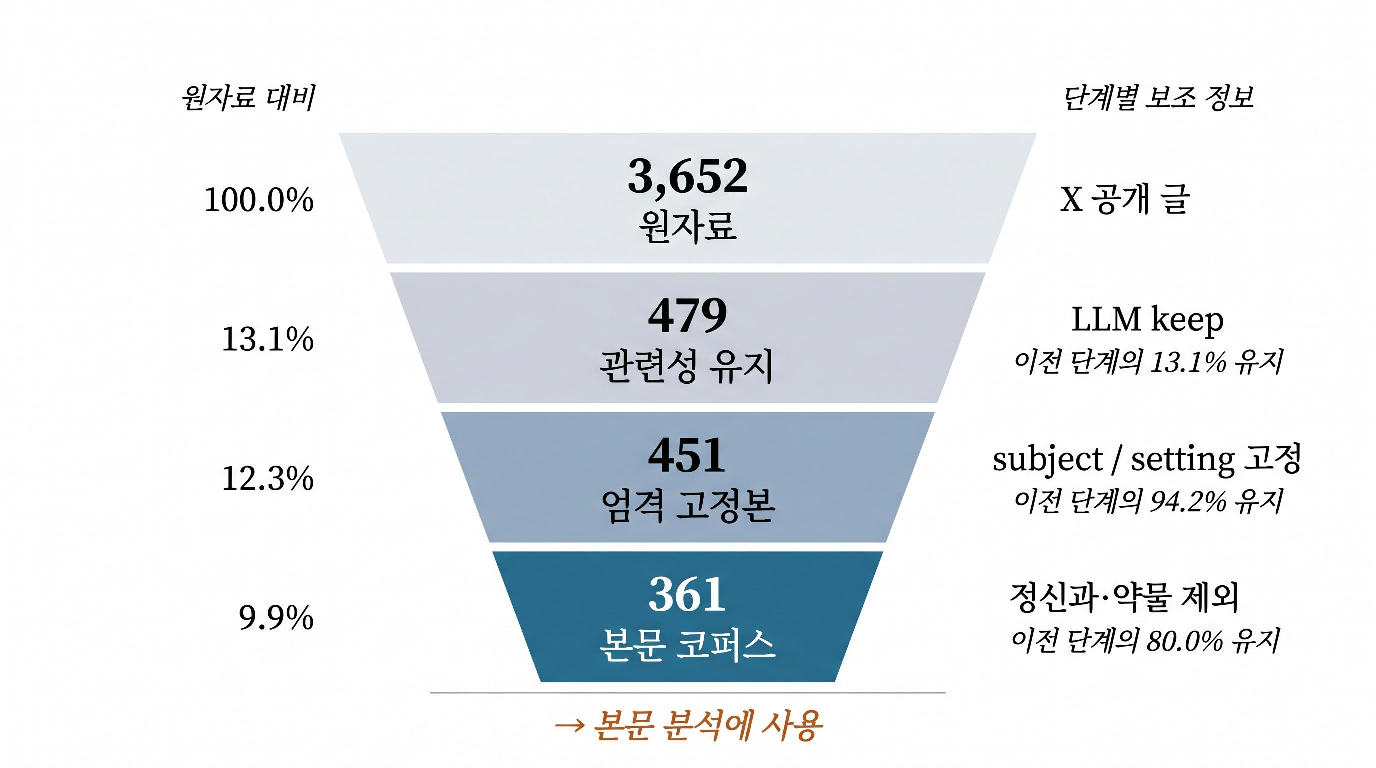
\includegraphics[width=188mm]{../figures/corpus_funnel.pdf}\end{center}
  \figcap{그림 2. 원자료 3{,}652건 $\rightarrow$ 본문 코퍼스 361건(9.9\%). 관련성 유지본 479$\cdot$엄격 확정본 451건 경유.}
\end{textblock}

% ===================== RIGHT COLUMN =====================
% IV. 연구결과
\begin{textblock}{338}(445,224)
  \fontsize{29}{38}\selectfont\justifying
  \subhd{기초 분포}
  본문 코퍼스 361건의 경험 극성은 부정 117$\cdot$혼합 91$\cdot$긍정 126$\cdot$중립 27건이다. 정식 표본에서 과소표집되던 부정 경험이 긍정과 엇비슷한 규모로 함께 들어왔다. 장면은 일반 정신건강 상담 268건과 청소년 학교상담 93건(약 26\%)으로 나뉘었다.
  \begin{center}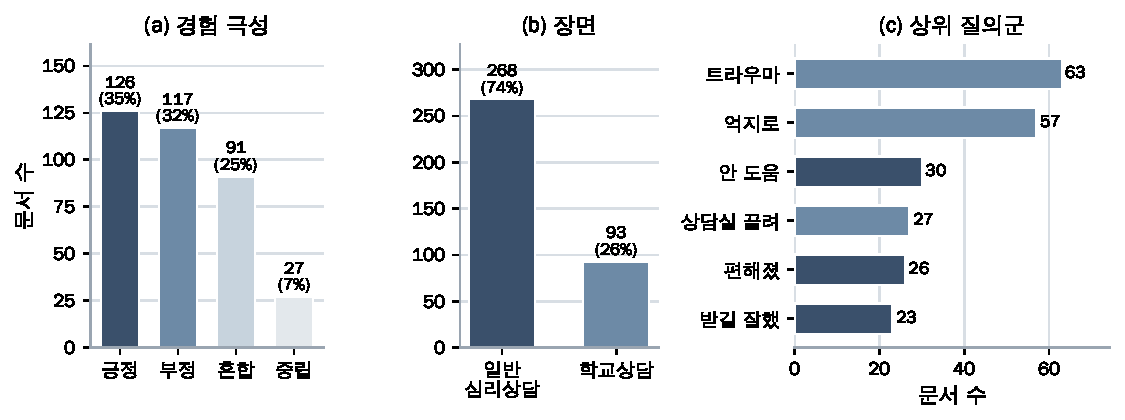
\includegraphics[width=318mm]{../figures/corpus_overview.pdf}\end{center}
  \figcap{그림 3. 본문 코퍼스 361건의 경험 극성$\cdot$장면$\cdot$상위 질의군 분포.}

  \subhd{면접 기반 선행 연구와의 비교}
  부정 117건에서 관찰된 사건 표지를 문보경$\cdot$장성숙(2001)의 면접 범주와 나란히 놓았다. 면접 자료에서 사건 단위로 정리된 부정 경험의 표지가 익명 환경의 글에서도 적용 가능한 형태로 드러난다.
  \vspace{2mm}

  {\fontsize{22}{29}\selectfont
  \setlength{\arrayrulewidth}{0.3pt}\arrayrulecolor{kcanavy!25}
  \renewcommand{\arraystretch}{1.45}
  \begin{tabularx}{\linewidth}{@{}>{\raggedright\arraybackslash}p{0.17\linewidth} >{\raggedright\arraybackslash}X >{\raggedright\arraybackslash}X@{}}
    \rowcolor{kcanavy}
    \textcolor{white}{\textbf{측면}} & \textcolor{white}{\textbf{면접 자료 (문보경$\cdot$장성숙, 2001)}} & \textcolor{white}{\textbf{본 SNS 자료}} \\
    \rowcolor{kcanavy!8}\textbf{자료원} & 내담자 면접$\cdot$개방형 질문지 & 한국어 공개 X 경험 글 \\
    \rowcolor{white}\textbf{분석 단위} & 사례 단위 사건 회고 & 게시물 단위 경험 글 \\
    \rowcolor{kcanavy!8}\textbf{부정 표지} & 원치 않는 반응, 해결책 부재, 상담자의 요구, 상처 경험 & 강제성 0.350, 무시당함 0.470, 상처 0.231 (부정 117건 기준) \\
    \rowcolor{white}\textbf{분석 깊이} & 사례별 깊이 있는 합의 부호화 & 분포 수준의 탐색적 부호화 \\
    \arrayrulecolor{kcanavy!40}\bottomrule
  \end{tabularx}}
  \figcap{표 1. 면접 기반 선행 연구와 본 SNS 자료의 분포 비교.}

  \subhd{과정 코드의 극성별 대비}
  작업동맹 세 축은 극성에 따라 갈렸다. 부정 117건에서는 유대 63.2\%$\cdot$과제 69.2\%$\cdot$목표 59.0\%가 부정 정렬, 긍정 126건에서는 유대 80.2\%$\cdot$과제 81.7\%$\cdot$목표 84.9\%가 긍정 정렬이었다. 여섯 과정 코드의 부트스트랩 대비는 신뢰구간이 모두 0을 가로지르지 않았다(예: 무시당함 $-0.431$ [$-0.506$, $-0.350$], 안도 $+0.434$ [$0.344$, $0.517$]).
  \begin{center}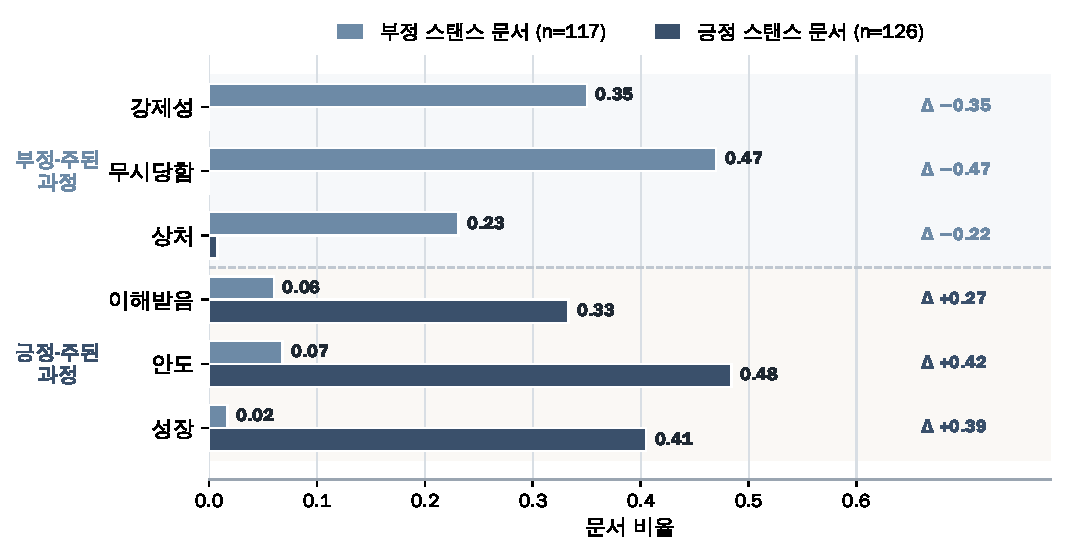
\includegraphics[width=318mm]{../figures/process_contrast.pdf}\end{center}
  \figcap{그림 4. 부정 경험(n=117)과 긍정 경험(n=126)의 과정 코드 대비.}
\end{textblock}

% V. 논의
\begin{textblock}{338}(445,938)
  \bodyfs\justifying
  \begin{itemize}
    \item \textbf{함의:} 정식 표본에서 좀처럼 함께 모이지 않던 부정과 긍정 경험이 익명 환경에서는 거의 같은 비중으로 함께 기록되었다(부정 117$\cdot$긍정 126건). 사건 단위의 경험 언어도 분포 수준에서 서로 구분되었으며, 그 표지는 면접 자료를 분석한 문보경$\cdot$장성숙(2001)과 닮았다. 다만 이 일치는 같은 모집단의 일치가 아니라, 본 연구의 코드가 그 표지를 출발점으로 삼은 데서 비롯한다.
    \item \textbf{한계:} 본 결과는 사람 합의 코딩층 없이 LLM 보조 부호화로만 얻었고, 익명 환경에서 자기 경험을 적는 사람이라는 표집 편향 위에서 관찰되었다.
    \item \textbf{전망:} 따라서 본 연구는 한국 상담 경험 일반에 대한 결론이 아닌 사례 보고이며, 후속 합의적 질적 연구와 면접$\cdot$SNS 직접 비교의 출발 자료로 쓸 수 있다.
  \end{itemize}
\end{textblock}

\end{document}
